%!TEX root = main.tex
\section{Precise Visual Querying\label{sec:precise}}
Visual analysis is valuable often reveal important -----. However, there are many -----. 

\subsection{Motivating Example}
Astronomers from the The Dark Energy Survey (DES)\cite{Drlica-Wagner2017} are interested in finding anomalous time series to discover astrophysical transients (objects whose brightness changes dramatically as a function of time), such as supernova explosions or quasars. When trying to find celestial objects corresponding to supernovae, which have a specific pattern of brightness over time, scientists need to individually inspect the visualizations of each object until they find ones that match the pattern. With more than 400 million objects in their catalog, each having their own set of time series brightness measurement, the process of manually exploring a large number of visualizations is not only error-prone, but also overwhelming for scientists who do not have extensive knowledge about their dataset.  
% Intention driven task-based querying (Precise search)
\par The astronomy use case highlights a common challenge in exploratory data analysis (EDA). There is often a large space of possible visualizations that could be generated from a given dataset and manual search through this large collection is inefficient.
%\par There has been many related work in this space varying different dimensions of possible visualizations, including visual encodings~\cite{showme}, data facets, . We will focus on 
There’s a large space of possibilities, manual search is tedious. Visualization authoring tools such as Tableau and Excel focusses on presenting one visualization at a time. There is no systematic way to create, compare, and query large collections of visualizations. 


Propose VQS as a solution\cite{Lee2017}. 

\subsection{Effortless Data Exploration with \zv}
\par The challenges presented earlier points to a need for a tool that enables users to create and search through large collections of visualizations. We developed \zv a visual query system that . \zv is built on top of a language ZQL offers a way to iterate over collections of visualizations. Different from grammar of graphics and others which focusses on encoding and viz\cite{Wongsuphasawat2016}, ZQL is a high-level specification. Iterate over collections of visualizations \cite{Siddiqui}. We demonstrate that -----, functionalities including: 
\begin{itemize}
	\item Comparing across a collection of visualizations by iterating over one or more x, y, z attributes while fixing other attributes (e.g. Find me all the cities where the housing prices starts off high then becomes lower over time. Here we vary along \textsc{city} while keeping \textsc{x=time,y=AVG(price)} fixed.)
	\item Finding the top-k visualizations whose y values are most or least similar from a queried visualization. 
	\item Finding a pair of X and Y axes where the visualizations for two specific products ‘stapler’ and ‘chair’ differ the most
\end{itemize}
\par Given a ZQL query, \zv parses it into a graph of visual component nodes(contains visualization information, such as X, Y columns) and task nodes (common and user-defined primitives for processing visual components, such as sort-filter). \zv then performs query optimization to merge together multiple nodes, as well as reducing the processing time required for individual visualization components. Using the optimized query plan, the executor compiles visual nodes into SQL queries for retreiving the visualization data and postprocesses the result via the defined operations. 
\par While ZQL provides powerful mechanism for expressively specifying queries on large collections visualizations, writing ZQL queries can be challenging for novice users. Therefore, we extracted a typical workflow of visualization querying (finding top-k most similar visualization from a collection with fixed X,Y while varying Z) to allow users to formulate ZQL queries through interactions (such as drag-and-drop, sketching), while allowing them to construct ZQL queries via a frontend table input if necessary.  we developed \zv frontend which leverages and authors ZQL queries --- full-fledged visual querying system that supports a variety of querying interactions as described in Figure~\ref{fig:modalities}. In the following section, we will discuss the design process of how we developed this visual query system and the lessons that we have learned in ---- visual data exploration systems.

\begin{figure}[h!]
\label{fig:modalities}
\centering
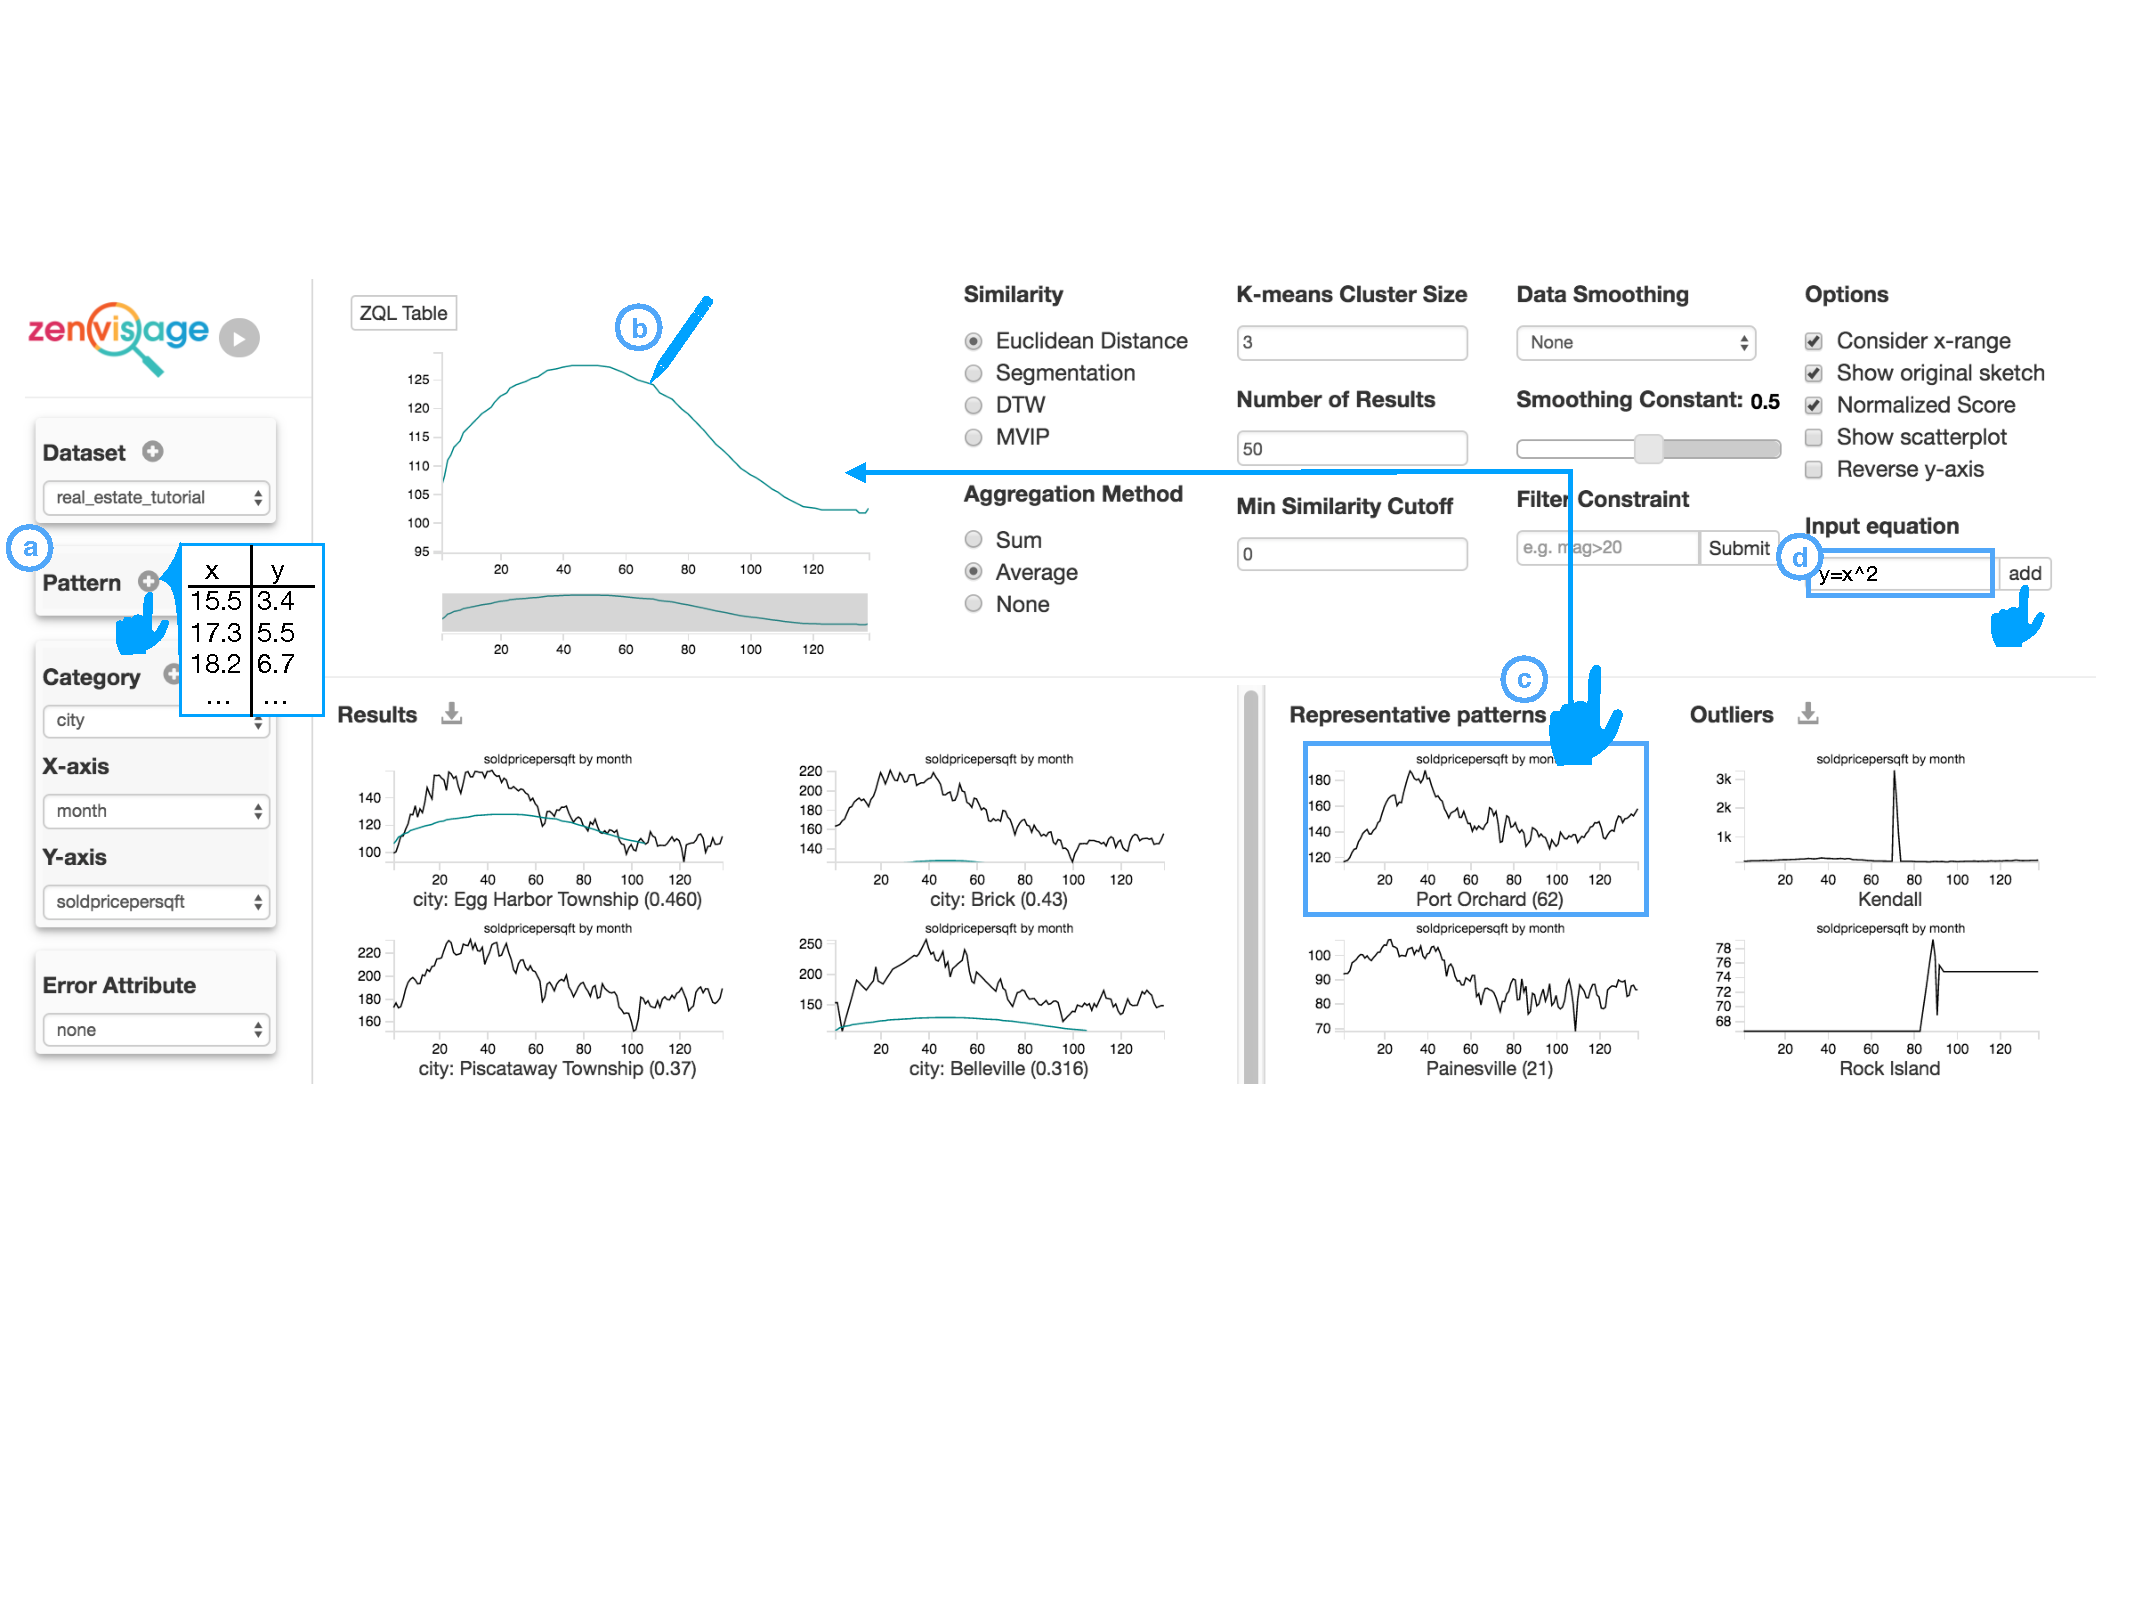
\includegraphics[width=0.8\textwidth]{figures/modalities.pdf}
\caption{\zv offers a variety of querying modalities, including: a) uploading a sample pattern from an external dataset as a query, b) sketching a query pattern, c) dragging-and-dropping an existing pattern from the dataset, and d) inputting an equation as a query.}
\end{figure}
